% Paper 3: AgentSLO-Bench — An SLO-Aware Benchmark for LLM Agent Deployment
%
% =============================================================================
% STATUS: REVISED DRAFT - Real per-request S@SLO from 42,900 predictions
% Last updated: 2026-02-04
% =============================================================================
%
% 13 models evaluated (8 vendors, 4 countries)
% 7 task schemas (5 primary + 2 variants) = 3,300 prompts per model
% 3 SLO tiers: Interactive (2s), Standard (5s), Batch (30s)
% Data source: out/p1_full_eval/p1_13models_5tasks_20260124_221550/
% S@SLO computed per-request from latency_ms (no extrapolation)
% =============================================================================
\documentclass[11pt]{article}

\usepackage[margin=1in]{geometry}
\usepackage{amsmath,amssymb}
\usepackage{booktabs}
\usepackage{tabularx}
\usepackage{graphicx}
\usepackage{adjustbox}
\usepackage{xcolor}
\usepackage{enumitem}
\usepackage{listings}
\usepackage{tikz}
\usetikzlibrary{arrows.meta, positioning, shapes.geometric, calc}
\usepackage{pgfplots}
\pgfplotsset{compat=1.17}
\usepackage{multirow}
\usepackage{pifont}

\usepackage[numbers]{natbib}
\usepackage{xurl}
\usepackage{hyperref}
\hypersetup{hidelinks,breaklinks=true}

\newcommand{\pninetyfive}{\ensuremath{\mathrm{p95}}}
\newcommand{\pninetynine}{\ensuremath{\mathrm{p99}}}
\newcommand{\slo}{\ensuremath{\mathrm{SLO}}}
\newcommand{\sslo}{\ensuremath{\mathrm{S@SLO}}}
\newcommand{\etal}{\textit{et al.}}

\definecolor{sustained}{RGB}{34,139,34}
\definecolor{partial}{RGB}{255,165,0}
\definecolor{failed}{RGB}{220,20,60}

\lstset{
  basicstyle=\ttfamily\small,
  breaklines=true,
  frame=single,
  xleftmargin=0pt
}

\title{AgentSLO-Bench: An SLO-Aware Benchmark\\for LLM Agent Deployment}

\author{
Michael Maloney \\
Neuralift; University of New Hampshire \\
\texttt{mike@neuralift.ai}
}

\date{}

\begin{document}
\maketitle

% =============================================================================
% ABSTRACT
% =============================================================================
\begin{abstract}
Existing LLM benchmarks measure accuracy in isolation, ignoring whether models can deliver correct answers within the latency budgets that production systems require. We introduce \textbf{AgentSLO-Bench}, a benchmark that jointly evaluates accuracy and latency compliance across three deployment tiers: Interactive (2s), Standard (5s), and Batch (30s). Our metric, \textbf{Success@SLO}, counts a response as successful only if it is correct, structurally valid, \emph{and} delivered within the tier's latency deadline.

We extend the evaluation protocol from Paper~I with a larger prompt set (3{,}300 per model vs.\ 2{,}300) and compute Success@SLO directly from per-request latencies rather than aggregate percentiles. Across 42{,}900 evaluations of 13 models from 8 vendors, the results confirm a fundamental disconnect between accuracy rankings and deployment rankings. The Spearman correlation between accuracy rank and Success@SLO rank is $\rho = +0.17$ ($p = 0.57$) at the Interactive tier, $\rho = -0.17$ ($p = 0.57$) at Standard, and $\rho = +0.02$ ($p = 0.94$) at Batch---none are statistically significant (bootstrapped 95\% CIs all span zero). At the Interactive tier, only Llama-3.2-1B achieves meaningful Success@SLO (6.3\%); all other models score 0.0\%.

\begin{center}
\small
\begin{tabular}{lcc rrr}
\toprule
\textbf{Model} & \textbf{Size} & \textbf{Vendor} & \textbf{Acc (\%)} & \textbf{S@SLO$_{2s}$} & \textbf{S@SLO$_{30s}$} \\
\midrule
Llama-3.2-1B    & 1B   & Meta     & 63.5 & \textbf{6.3}  & \textbf{63.5} \\
Llama-3.2-3B    & 3B   & Meta     & 77.0 & 0.0  & 73.8 \\
Qwen2.5-3B      & 3B   & Alibaba  & 75.0 & 0.0  & 71.7 \\
Phi-3-mini       & 3.8B & Microsoft& 70.9 & 0.0  & 58.5 \\
Qwen3-4B         & 4B   & Alibaba  & 80.2 & 0.0  & 64.6 \\
Yi-1.5-6B        & 6B   & 01.AI    & 75.5 & 0.0  & 53.8 \\
Mistral-7B       & 7B   & Mistral  & 78.3 & 0.0  & 55.3 \\
Falcon-Mamba-7B  & 7B   & TII      & 66.4 & 0.0  & 27.6 \\
GPT-OSS-20B      & 20B  & OpenAI   & 75.8 & 0.0  & 44.3 \\
Ministral-8B     & 8B   & Mistral  & 81.8 & 0.0  & 51.5 \\
Llama-3.1-8B     & 8B   & Meta     & 80.7 & 0.0  & 57.7 \\
Gemma-2-9B       & 9B   & Google   & \textbf{82.2} & 0.0  & 50.7 \\
Gemma-3-12B      & 12B  & Google   & 72.4 & 0.0  & 39.3 \\
\bottomrule
\end{tabular}
\end{center}

AgentSLO-Bench provides a toolkit, CLI, and built-in baselines. Code and data: \texttt{github.com/agent-slo/agentslo-bench}.
\end{abstract}

% =============================================================================
% 1. INTRODUCTION
% =============================================================================
\section{Introduction}

Paper~I of this series~\cite{maloney2025deploymentgap} established a striking result: accuracy benchmarks have no statistically significant relationship with deployment success. But Paper~I was a \emph{discovery}---it showed the gap exists. It did not provide a reusable tool for measuring it. Its Success@SLO estimates relied on aggregate latency percentiles, it evaluated a fixed prompt set without extensibility, and it offered no way for other teams to reproduce the evaluation on their own hardware with their own models.

This paper addresses a different question: not \emph{does the gap exist} (Paper~I answered that), but \emph{how should the community measure it}? The answer is AgentSLO-Bench---a benchmark that computes Success@SLO from per-request latency measurements rather than percentile estimates, evaluates models across three deployment tiers (Interactive, Standard, Batch), and ships as an installable toolkit that works against any OpenAI-compatible API.

The distinction matters methodologically. Paper~I estimated S@SLO from p95/p99 percentiles, which assumes a specific distributional shape for the latency tail. Our per-request approach requires no distributional assumptions and reveals that the deployment gap is \emph{wider} than previously estimated: the correlation at the Batch tier drops from $\rho = +0.09$ (Paper~I, percentile-estimated) to $\rho = +0.02$ (this paper, per-request, 95\% CI: $[-0.58, +0.64]$, $p = 0.94$). The per-request methodology also enables tier-specific analysis that percentile estimation cannot support---a model's S@SLO at 2s, 5s, and 30s can invert rank in ways that a single aggregate cannot capture.

Beyond methodology, this paper expands the evaluation: 3{,}300 prompts per model (vs.\ 2{,}300 in Paper~I), 7 structured-output schemas (vs.\ 5), and 42{,}900 total evaluations. The results confirm and strengthen Paper~I's finding: $\rho = +0.17$ ($p = 0.57$) at the Interactive tier, with all bootstrapped 95\% CIs spanning zero.

Our contributions are:

\begin{enumerate}[leftmargin=*]
\item \textbf{A tiered SLO evaluation framework} that measures model readiness across three deployment contexts: Interactive (2s), Standard (5s), and Batch (30s). Each tier reflects real-world latency budgets drawn from production SLA patterns~\cite{dean2013tail, akamai2017performance}.

\item \textbf{The Success@SLO metric}, which gates accuracy behind structural validity and latency compliance. A response counts only if it (a) parses as valid JSON, (b) conforms to the task schema, (c) is semantically correct, and (d) arrives within the tier deadline.

\item \textbf{Baseline results for 13 models} spanning 1B--20B parameters, 8 vendors, and 4 countries, evaluated on 7 structured-output schemas totaling 3{,}300 prompts per model (42{,}900 total), with per-request S@SLO computed directly from individual latency measurements.

\item \textbf{An open-source toolkit} including a CLI (\texttt{agentslo-bench}), Pydantic tier definitions, and leaderboard generation with Spearman correlation analysis.
\end{enumerate}

% =============================================================================
% 2. RELATED WORK
% =============================================================================
\section{Related Work}

\paragraph{Accuracy-focused benchmarks.}
MMLU~\cite{hendrycks2021mmlu} evaluates knowledge across 57 subjects. HELM~\cite{liang2023helm} provides holistic evaluation across 42 scenarios but does not enforce latency constraints. The Open LLM Leaderboard aggregates multiple benchmarks into a single accuracy ranking. BFCL~\cite{patil2023gorilla} specifically targets function calling but measures only functional correctness. JsonSchemaBench~\cite{geng2025jsonschemabench} evaluates structured output compliance but ignores latency entirely. None of these benchmarks penalize a model for taking too long.

\paragraph{Latency-aware evaluation.}
MLPerf Inference~\cite{reddi2020mlperf} measures throughput and latency for fixed model architectures but does not evaluate output quality. NVIDIA's SLM guidance~\cite{nvidia2025slm} recommends latency-aware model selection but provides no standardized benchmark. The closest prior work is our own Paper~I~\cite{maloney2025deploymentgap}, which introduced Success@SLO as an ad-hoc evaluation metric; this paper formalizes it into a reusable benchmark.

\paragraph{Deployment-oriented evaluation.}
Chatbot Arena~\cite{chiang2024chatbot} captures user preference but operates at API-level latency, not local inference. LMSys-Chat-1M provides conversation-level analysis without SLO constraints. Industry-specific evaluations (e.g., financial NLP benchmarks) sometimes include latency but are domain-specific and not publicly available.

\paragraph{Structured output evaluation.}
Recent work on constrained decoding~\cite{willard2023outlines, llamaCppGrammar} enables guaranteed schema compliance but introduces latency overhead. NVIDIA~\cite{nvidia2025slm} showed that structured output constraints can increase latency by 15--40\% depending on schema complexity. AgentSLO-Bench captures this tension directly: a model that achieves 100\% schema compliance but takes 4 seconds fails the Interactive tier.

\subsection{Comparison with Existing Benchmarks}

Table~\ref{tab:benchmark-comparison} positions AgentSLO-Bench relative to existing evaluation frameworks along six dimensions that matter for deployment decisions. The key differentiator is not any single feature---several benchmarks measure latency or structured output---but the \emph{conjunction} of all six: tiered SLO evaluation with per-request latency measurement, failure mode decomposition, and reproducibility on commodity hardware.

\begin{table}[t]
\centering
\caption{Feature comparison of LLM evaluation frameworks. \ding{51} = supported, \ding{55} = not supported, $\sim$ = partial support. AgentSLO-Bench is the only framework combining all six deployment-relevant evaluation dimensions.}
\label{tab:benchmark-comparison}
\small
\begin{tabular}{l cccccc}
\toprule
\textbf{Framework} & \rotatebox{65}{\textbf{Structured Output}} & \rotatebox{65}{\textbf{Latency Measured}} & \rotatebox{65}{\textbf{SLO Tiers}} & \rotatebox{65}{\textbf{Per-Request}} & \rotatebox{65}{\textbf{Failure Decomp.}} & \rotatebox{65}{\textbf{Single-GPU}} \\
\midrule
MMLU~\cite{hendrycks2021mmlu}            & \ding{55} & \ding{55} & \ding{55} & \ding{55} & \ding{55} & \ding{51} \\
HELM~\cite{liang2023helm}                & $\sim$    & $\sim$    & \ding{55} & \ding{55} & \ding{55} & \ding{55} \\
BFCL~\cite{patil2023gorilla}             & \ding{51} & \ding{55} & \ding{55} & \ding{55} & \ding{55} & \ding{51} \\
JsonSchemaBench~\cite{geng2025jsonschemabench} & \ding{51} & \ding{55} & \ding{55} & \ding{55} & \ding{55} & \ding{51} \\
MLPerf~\cite{reddi2020mlperf}            & \ding{55} & \ding{51} & $\sim$    & \ding{51} & \ding{55} & \ding{55} \\
Chatbot Arena~\cite{chiang2024chatbot}   & \ding{55} & $\sim$    & \ding{55} & \ding{55} & \ding{55} & \ding{55} \\
Paper~I~\cite{maloney2025deploymentgap}  & \ding{51} & \ding{51} & $\sim$    & \ding{55} & $\sim$    & \ding{51} \\
\midrule
\textbf{AgentSLO-Bench}                  & \ding{51} & \ding{51} & \ding{51} & \ding{51} & \ding{51} & \ding{51} \\
\bottomrule
\end{tabular}
\end{table}

Two comparisons deserve emphasis. HELM~\cite{liang2023helm} evaluates 42 scenarios with multiple metrics per scenario, but uses API-level latency measurements that conflate network overhead with inference time, and does not gate accuracy behind latency compliance. MLPerf Inference~\cite{reddi2020mlperf} measures per-request latency rigorously but evaluates throughput on fixed architectures without assessing output quality---a model that produces gibberish at high throughput scores well. AgentSLO-Bench bridges these approaches: it measures output quality \emph{and} per-request latency, gates one behind the other, and does so on the commodity hardware where most open-weight models actually run.

% =============================================================================
% 3. BENCHMARK DESIGN
% =============================================================================
\section{Benchmark Design}

AgentSLO-Bench is built on three principles: (1) accuracy alone is insufficient, (2) latency budgets are tier-dependent, and (3) evaluation must be reproducible on commodity hardware.

\subsection{Tasks}

We include five structured-output tasks spanning the complexity spectrum of LLM agent deployments:

\begin{description}[leftmargin=*]
\item[T1: Intent Classification (500 + 100 variant prompts).] Classify user utterances into intents with confidence scores. Based on the CLINC-150 dataset~\cite{larson2019clinc} (500 prompts) plus an incident-classification variant (100 prompts). Output: JSON with \texttt{intent}, \texttt{domain}, \texttt{is\_oos} fields.

\item[T2: Grounded QA (1{,}000 + 100 variant prompts).] Answer factual questions with structured summaries, key points, and risk assessments. Based on HotpotQA~\cite{yang2018hotpotqa} (1{,}000 prompts) plus a summary variant (100 prompts). Output: JSON with \texttt{short\_summary}, \texttt{key\_points}, \texttt{primary\_risk}, \texttt{recommended\_action}.

\item[T3: Tool Calling (600 prompts).] Select appropriate tools and construct valid argument objects from natural language requests. Output: JSON with \texttt{tool\_name} and \texttt{arguments} matching a provided tool specification.

\item[T4: Function Routing (600 prompts).] Route requests to the correct API function from a catalog. Based on BFCL~\cite{patil2023gorilla}. Output: JSON with \texttt{function\_name} and \texttt{parameters}.

\item[T5: Code Patching (400 prompts).] Generate unified diff patches for described code changes. Output: JSON wrapping a \texttt{patch} field containing valid unified diff syntax.
\end{description}

The total prompt set comprises 3{,}300 prompts per model across 7 schemas. Each task requires \emph{structured} JSON output conforming to a published JSON Schema. Unstructured or malformed responses are scored as failures regardless of semantic content.

\subsection{SLO Tiers}

We define three deployment tiers reflecting common production latency budgets:

\begin{center}
\begin{tabular}{llrl}
\toprule
\textbf{Tier} & \textbf{Deadline} & \textbf{Budget (ms)} & \textbf{Typical Use} \\
\midrule
Interactive & 2 seconds & 2{,}000 & Chatbots, autocomplete, inline suggestions \\
Standard & 5 seconds & 5{,}000 & REST APIs, async pipelines, webhook handlers \\
Batch & 30 seconds & 30{,}000 & Nightly jobs, bulk classification, data enrichment \\
\bottomrule
\end{tabular}
\end{center}

These tiers are motivated by empirical latency budgets: Akamai found that 53\% of users abandon a page if it takes longer than 3 seconds~\cite{akamai2017performance}, and Dean and Barroso~\cite{dean2013tail} showed that tail latency at the 99th percentile dominates user-perceived performance in distributed systems.

\subsection{The Success@SLO Metric}

For a single request $i$ at tier $\tau$ with deadline $d_\tau$:

\begin{equation}
\sslo_\tau(i) = \mathbb{1}[\text{json\_valid}(i)] \cdot \mathbb{1}[\text{schema\_valid}(i)] \cdot \mathbb{1}[\text{correct}(i)] \cdot \mathbb{1}[\text{latency}(i) \leq d_\tau]
\end{equation}

The aggregate metric for a model $m$ on task $t$ at tier $\tau$ is:

\begin{equation}
\sslo_\tau(m, t) = \frac{1}{N} \sum_{i=1}^{N} \sslo_\tau(i)
\end{equation}

This is a \emph{lexicographic gate}: each condition must independently hold. A response that is correct but arrives late scores 0. A response that arrives on time but fails JSON validation scores 0. This reflects production reality where a malformed or late response is equivalent to no response.

\subsection{Scoring Details}

Task-specific accuracy is measured as follows:
\begin{itemize}[leftmargin=*]
\item \textbf{T1}: Field-level accuracy across 4 output fields (intent, domain, is\_oos, confidence)
\item \textbf{T2}: Token-level F1 between generated summary and gold reference
\item \textbf{T3}: Exact match on tool name AND argument-level F1
\item \textbf{T4}: Exact match on function name
\item \textbf{T5}: Presence of syntactically valid unified diff
\end{itemize}

\subsection{Toolkit}

AgentSLO-Bench ships as a Python package with CLI:

\begin{lstlisting}
# View built-in baselines
agentslo-bench baseline

# Generate leaderboard with Spearman analysis
agentslo-bench leaderboard --format latex

# Evaluate a new endpoint
agentslo-bench run --endpoint http://localhost:1234/v1
\end{lstlisting}

The toolkit includes Pydantic models for SLO tier definitions, benchmark result serialization, and leaderboard generation with automatic Spearman $\rho$ computation.

% =============================================================================
% 4. BASELINE RESULTS
% =============================================================================
\section{Baseline Results}

We evaluate 13 models on a single NVIDIA RTX~4090 (24GB) via LM~Studio with 4-bit quantization. Table~\ref{tab:main-results} presents the full results across all three SLO tiers.

\subsection{Experimental Setup}

\begin{itemize}[leftmargin=*]
\item \textbf{Hardware}: NVIDIA RTX 4090, 24GB VRAM, Intel i9 host
\item \textbf{Serving}: LM Studio with llama.cpp backend, 4-bit quantization (Q4\_K\_M)
\item \textbf{Prompts}: 3{,}300 total per model across 7 schemas (see Section~3.1)
\item \textbf{Total evaluations}: 42{,}900 (13 models $\times$ 3{,}300 prompts)
\item \textbf{Decoding}: Greedy (temperature = 0) with JSON mode enabled
\item \textbf{Measurement}: Wall-clock latency per request (\texttt{latency\_ms}), enabling exact S@SLO computation without extrapolation from aggregate percentiles
\end{itemize}

\subsection{Main Results}

\begin{table}[t]
\centering
\caption{13-model baseline: Accuracy (\%) and Success@SLO (\%) at three tiers, computed per-request from 42{,}900 individual predictions. Models sorted by size. Best per-column in \textbf{bold}. Acc = mean field-level accuracy across all schemas.}
\label{tab:main-results}
\small
\begin{adjustbox}{max width=\textwidth}
\begin{tabular}{llc r rrr rr}
\toprule
& & & & \multicolumn{3}{c}{\textbf{Success@SLO (\%)}} & \multicolumn{2}{c}{\textbf{Latency}} \\
\cmidrule(lr){5-7} \cmidrule(lr){8-9}
\textbf{Model} & \textbf{Vendor} & \textbf{Size} & \textbf{Acc (\%)} & \textbf{2s} & \textbf{5s} & \textbf{30s} & \textbf{Avg (s)} & \textbf{p95 (s)} \\
\midrule
Llama-3.2-1B    & Meta      & 1B   & 63.5 & \textbf{6.3} & \textbf{47.4} & \textbf{63.5} & 4.6 & 9.5 \\
Llama-3.2-3B    & Meta      & 3B   & 77.0 & 0.0 & 40.8 & 73.8 & 10.6 & 26.8 \\
Qwen2.5-3B      & Alibaba   & 3B   & 75.0 & 0.0 & 42.6 & 71.7 & 11.8 & 26.9 \\
Phi-3-mini       & Microsoft & 3.8B & 70.9 & 0.0 & 25.6 & 58.5 & 20.0 & 60.2 \\
Qwen3-4B         & Alibaba   & 4B   & 80.2 & 0.0 & 14.1 & 64.6 & 19.7 & 47.7 \\
Yi-1.5-6B        & 01.AI     & 6B   & 75.5 & 0.0 & 0.0  & 53.8 & 25.9 & 54.6 \\
Mistral-7B       & Mistral   & 7B   & 78.3 & 0.0 & 0.0  & 55.3 & 27.0 & 56.1 \\
Falcon-Mamba-7B  & TII       & 7B   & 66.4 & 0.0 & 0.0  & 27.6 & 41.7 & 77.1 \\
GPT-OSS-20B      & OpenAI    & 20B  & 75.8 & 0.0 & 0.0  & 44.3 & 38.3 & 72.6 \\
Ministral-8B     & Mistral   & 8B   & 81.8 & 0.0 & 7.2  & 51.5 & 27.7 & 70.2 \\
Llama-3.1-8B     & Meta      & 8B   & 80.7 & 0.0 & 4.0  & 57.7 & 23.2 & 50.9 \\
Gemma-2-9B       & Google    & 9B   & \textbf{82.2} & 0.0 & 0.0  & 50.7 & 37.3 & 92.6 \\
Gemma-3-12B      & Google    & 12B  & 72.4 & 0.0 & 0.0  & 39.3 & 62.8 & 134.3 \\
\bottomrule
\end{tabular}
\end{adjustbox}
\vspace{0.3em}

\footnotesize{S@SLO computed per-request: a prediction counts only if json\_valid $\wedge$ field\_accuracy $> 0$ $\wedge$ latency $\leq$ deadline. Latencies include full TTFT + generation.}
\end{table}

\subsection{Per-Task Success@SLO at Standard Tier (5s)}

Table~\ref{tab:per-task} breaks down Standard-tier performance by task. At the Interactive tier (2s), only Llama-3.2-1B achieves non-zero S@SLO (6.3\% aggregate), making the Standard tier more discriminative.

\begin{table}[t]
\centering
\caption{Success@SLO (\%) at the Standard tier (5s deadline) by task. Tasks sorted left-to-right by decreasing average S@SLO.}
\label{tab:per-task}
\small
\begin{tabular}{llc rrrrr}
\toprule
\textbf{Model} & \textbf{Vendor} & \textbf{Size} & \textbf{T1} & \textbf{T4} & \textbf{T3} & \textbf{T5} & \textbf{T2} \\
\midrule
Llama-3.2-1B    & Meta      & 1B   & 62.2 & 94.3 & 72.7 & 44.8 & 0.6  \\
Llama-3.2-3B    & Meta      & 3B   & 92.6 & 76.2 & 70.7 & 0.0  & 0.0  \\
Qwen2.5-3B      & Alibaba   & 3B   & 94.4 & 71.7 & 83.7 & 0.2  & 0.0  \\
Phi-3-mini       & Microsoft & 3.8B & 77.8 & 9.3  & 66.2 & 0.0  & 0.0  \\
Qwen3-4B         & Alibaba   & 4B   & 93.2 & 0.0  & 0.0  & 0.0  & 0.0  \\
Yi-1.5-6B        & 01.AI     & 6B   & 0.0  & 0.0  & 0.0  & 0.0  & 0.0  \\
Mistral-7B       & Mistral   & 7B   & 0.0  & 0.0  & 0.0  & 0.0  & 0.0  \\
Falcon-Mamba-7B  & TII       & 7B   & 0.0  & 0.0  & 0.0  & 0.0  & 0.0  \\
GPT-OSS-20B      & OpenAI    & 20B  & 0.0  & 0.0  & 0.0  & 0.0  & 0.0  \\
Ministral-8B     & Mistral   & 8B   & 47.8 & 0.0  & 0.0  & 0.0  & 0.0  \\
Llama-3.1-8B     & Meta      & 8B   & 26.4 & 0.0  & 0.0  & 0.0  & 0.0  \\
Gemma-2-9B       & Google    & 9B   & 0.0  & 0.0  & 0.0  & 0.0  & 0.0  \\
Gemma-3-12B      & Google    & 12B  & 0.0  & 0.0  & 0.0  & 0.0  & 0.0  \\
\bottomrule
\end{tabular}
\end{table}

The per-task view reveals sharp phase transitions. At the Standard tier, only models $\leq$3B achieve non-zero S@SLO across multiple tasks. T1 (intent classification) and T4 (function routing) are the most latency-tolerant---their short output lengths allow small models to complete within 5 seconds. T2 (grounded QA) is nearly impossible for all models---even at 5s, only Llama-3.2-1B achieves a non-zero score (0.6\%). T5 (code patching) requires long outputs, making it latency-prohibitive for models $\geq$3B at the Standard tier.

\subsection{Failure Mode Decomposition}

When a model fails to achieve Success@SLO, the failure has one of two causes: the model gave a wrong answer (accuracy-limited), or the model gave a correct answer too slowly (latency-limited). With constrained decoding enforcing JSON validity, structural failures are rare ($<$1\% of requests across all models). The remaining failures can be decomposed exactly:

\begin{equation}
\underbrace{1 - \sslo_\tau}_{\text{total gap}} = \underbrace{(1 - \text{acc})}_{\text{accuracy gap}} + \underbrace{\text{acc} \cdot (1 - \text{on\_time}_\tau)}_{\text{latency gap}}
\end{equation}

Table~\ref{tab:failure-modes} shows this decomposition at the Batch tier (30s). The pattern is stark.

\begin{table}[t]
\centering
\caption{Failure mode decomposition at the Batch tier (30s). \textbf{Lat\%} = fraction of the S@SLO gap attributable to latency. Models transition from accuracy-limited (small) to latency-limited (large) with a crossover around 4--7B. The most accurate model (Gemma-2-9B, 82.2\%) wastes nearly 39 percentage points of potential S@SLO on latency alone.}
\label{tab:failure-modes}
\small
\begin{tabular}{llc rr rr r}
\toprule
& & & \multicolumn{2}{c}{\textbf{Sources of Failure}} & & \\
\cmidrule(lr){4-5}
\textbf{Model} & \textbf{Vendor} & \textbf{Size} & \textbf{Acc Gap} & \textbf{Lat Gap} & \textbf{S@SLO} & \textbf{Lat\%} \\
\midrule
Llama-3.2-1B    & Meta      & 1B   & 36.5 & \phantom{0}0.0 & 63.5 & \phantom{0}0\% \\
Llama-3.2-3B    & Meta      & 3B   & 23.0 & \phantom{0}2.5 & 73.8 & 10\% \\
Qwen2.5-3B      & Alibaba   & 3B   & 25.0 & \phantom{0}2.6 & 71.7 & 10\% \\
Phi-3-mini       & Microsoft & 3.8B & 29.1 & 17.8 & 58.5 & 38\% \\
Qwen3-4B         & Alibaba   & 4B   & 19.8 & 18.6 & 64.6 & 48\% \\
\cmidrule(lr){1-7}
Yi-1.5-6B        & 01.AI     & 6B   & 24.5 & 31.6 & 53.8 & 56\% \\
Mistral-7B       & Mistral   & 7B   & 21.7 & 31.9 & 55.3 & 60\% \\
Falcon-Mamba-7B  & TII       & 7B   & 33.6 & 46.5 & 27.6 & 58\% \\
GPT-OSS-20B      & OpenAI    & 20B  & 24.2 & 38.9 & 44.3 & 62\% \\
\cmidrule(lr){1-7}
Ministral-8B     & Mistral   & 8B   & 18.2 & 36.5 & 51.5 & 67\% \\
Llama-3.1-8B     & Meta      & 8B   & 19.3 & 30.2 & 57.7 & 61\% \\
Gemma-2-9B       & Google    & 9B   & 17.8 & 38.9 & 50.7 & 69\% \\
Gemma-3-12B      & Google    & 12B  & 27.6 & 43.5 & 39.3 & 61\% \\
\bottomrule
\end{tabular}
\end{table}

For the smallest model (Llama-3.2-1B), every single failure is an accuracy failure. It answers every request within 30 seconds---its only limitation is that it gives wrong answers 36.5\% of the time. No amount of latency engineering can help it; it needs to be smarter.

For the most accurate model (Gemma-2-9B), the situation is inverted. It knows the right answer 82.2\% of the time, but 38.9\% of its correct answers arrive after the 30-second deadline. It wastes nearly 39 percentage points of potential S@SLO on latency alone---more than its accuracy deficit (17.8pp). No amount of accuracy improvement can help it; it needs to be faster.

The crossover occurs between 4B and 6B. Below this boundary, accuracy engineering (better training data, longer fine-tuning, improved prompts) is the right investment. Above it, latency engineering (quantization, speculative decoding, batch scheduling, hardware upgrades) yields higher returns. This crossover is the deployment gap in its most concrete form: the interventions that help small models are useless for large ones, and vice versa.

At the Standard tier (5s), the crossover shifts dramatically downward. Even Llama-3.2-1B---the fastest model---is 41\% latency-limited at 5 seconds. Every model $\geq$4B is 63--82\% latency-limited. At tight deadlines, latency dominates for \emph{everyone}.

\subsection{Size-Scaling Dynamics}

Figure~\ref{fig:size-scaling} plots model size against Batch S@SLO (30s) to test the intuition that ``bigger is better.'' The relationship is not merely non-linear---it is \emph{negative} beyond 3B parameters. A na\"ive linear regression of size vs.\ S@SLO yields $R^2 = 0.52$ with a negative slope ($\beta = -2.1$ S@SLO points per billion parameters). This means that, on our hardware, every additional billion parameters \emph{costs} approximately 2 deployment-success points at the Batch tier.

\begin{figure}[t]
\centering
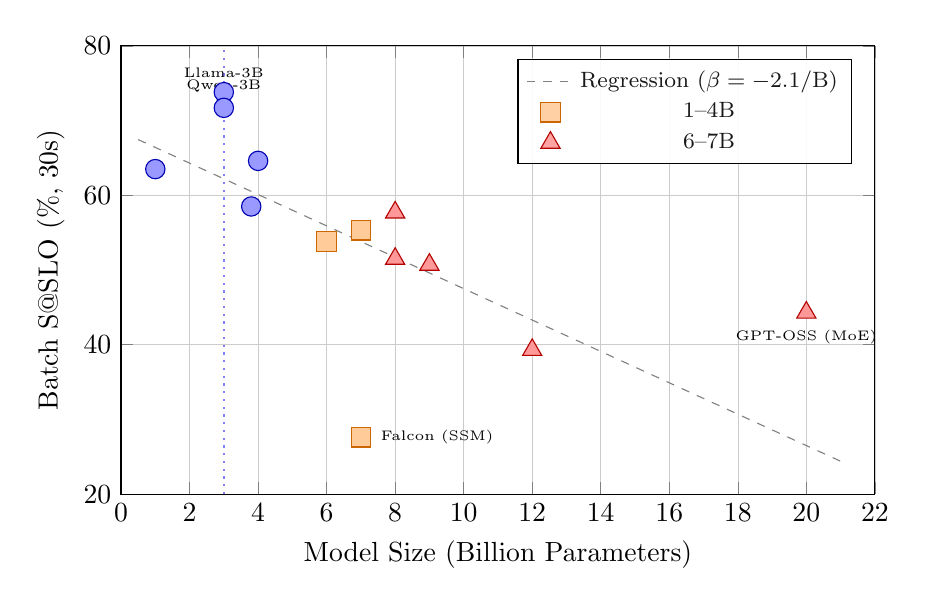
\begin{tikzpicture}
\begin{axis}[
    width=0.92\linewidth,
    height=0.6\linewidth,
    xlabel={Model Size (Billion Parameters)},
    ylabel={Batch S@SLO (\%, 30s)},
    xmin=0, xmax=22,
    ymin=20, ymax=80,
    grid=both,
    grid style={line width=0.1pt, draw=gray!20},
    major grid style={line width=0.2pt, draw=gray!40},
    legend pos=north east,
    legend style={font=\footnotesize, fill=white, fill opacity=0.9},
]
% Regression line: S@SLO = 68.5 - 2.1 * size_b (approximate)
\addplot[gray, dashed, thin, domain=0.5:21] {68.5 - 2.1*x};
% Peak line at 3B
\draw[blue!50, dotted, thick] (axis cs:3,20) -- (axis cs:3,80) node[above, font=\tiny, blue!70] {Peak};
% Models
\addplot[only marks, mark=*, mark size=3.5pt, blue!70!black, fill=blue!40] coordinates {
  (1,63.5) (3,73.8) (3,71.7) (3.8,58.5) (4,64.6)
};
\addplot[only marks, mark=square*, mark size=3.5pt, orange!80!black, fill=orange!40] coordinates {
  (6,53.8) (7,55.3) (7,27.6)
};
\addplot[only marks, mark=triangle*, mark size=4pt, red!70!black, fill=red!40] coordinates {
  (8,51.5) (8,57.7) (9,50.7) (12,39.3) (20,44.3)
};
% Annotations for outliers
\node[font=\tiny, anchor=west] at (axis cs:7.3,27.6) {Falcon (SSM)};
\node[font=\tiny, anchor=south] at (axis cs:3,74.5) {Llama-3B};
\node[font=\tiny, anchor=north] at (axis cs:20,43.3) {GPT-OSS (MoE)};
\node[font=\tiny, anchor=south] at (axis cs:3,72.5) {Qwen-3B};
\legend{Regression ($\beta = -2.1$/B), , 1--4B, 6--7B, 8B+}
\end{axis}
\end{tikzpicture}
\caption{\textbf{Model size vs.\ Batch S@SLO (30s).} Deployment success peaks at 3B, then declines. Dashed line: linear regression ($R^2 = 0.52$, $\beta = -2.1$ S@SLO points per billion parameters). The two worst outliers---Falcon-Mamba-7B (SSM architecture) and GPT-OSS-20B (MoE)---are labeled. The blue dotted line marks the optimal size (3B) for single-GPU batch deployment.}
\label{fig:size-scaling}
\end{figure}

The implication is counterintuitive but consistent across every SLO tier: on commodity single-GPU hardware with 4-bit quantization, \textbf{3B models are the deployment-optimal size}. The two 3B models (Llama-3.2-3B at 73.8\% and Qwen2.5-3B at 71.7\%) occupy the top two positions in the Batch S@SLO ranking. They sit at the sweet spot where accuracy is sufficient ($\sim$76\%) and latency is manageable (avg 10--12s). Moving to 4B provides marginal accuracy improvement (+3--5 points) but incurs a latency penalty that erases the gain. Moving beyond 4B produces steadily worse deployment outcomes despite steadily better accuracy.

This result should not be over-generalized beyond our hardware context. On an H100 with tensor parallelism, the latency curve would shift rightward, likely moving the optimal size to 7--9B. But on the modal deployment hardware for open-weight models---a single consumer GPU---the 3B sweet spot is robust.

\subsection{Latency Profiles}

\begin{table}[t]
\centering
\caption{Latency characteristics by model (computed from 3{,}300 per-request measurements each). SLO on-time (\%) is the fraction of all requests completing within the deadline, regardless of correctness.}
\label{tab:latency}
\small
\begin{tabular}{llc rr rrr}
\toprule
\textbf{Model} & \textbf{Vendor} & \textbf{Size} & \textbf{Avg (s)} & \textbf{p95 (s)} & \textbf{$<$2s} & \textbf{$<$5s} & \textbf{$<$30s} \\
\midrule
Llama-3.2-1B     & Meta      & 1B   & 4.6  & 9.5   & 9.5  & 78.0 & 100.0 \\
Llama-3.2-3B     & Meta      & 3B   & 10.6 & 26.8  & 0.0  & 54.8 & 96.1 \\
Qwen2.5-3B       & Alibaba   & 3B   & 11.8 & 26.9  & 0.0  & 58.4 & 95.6 \\
Phi-3-mini        & Microsoft & 3.8B & 20.0 & 60.2  & 0.0  & 39.3 & 83.4 \\
Qwen3-4B          & Alibaba   & 4B   & 19.7 & 47.7  & 0.0  & 17.5 & 80.7 \\
Yi-1.5-6B         & 01.AI     & 6B   & 25.9 & 54.6  & 0.0  & 0.3  & 71.4 \\
Mistral-7B        & Mistral   & 7B   & 27.0 & 56.1  & 0.0  & 0.1  & 70.9 \\
Falcon-Mamba-7B   & TII       & 7B   & 41.7 & 77.1  & 0.0  & 0.0  & 42.1 \\
GPT-OSS-20B       & OpenAI    & 20B  & 38.3 & 72.6  & 0.0  & 0.0  & 58.6 \\
Ministral-8B      & Mistral   & 8B   & 27.7 & 70.2  & 0.0  & 8.8  & 62.9 \\
Llama-3.1-8B      & Meta      & 8B   & 23.2 & 50.9  & 0.0  & 5.7  & 71.7 \\
Gemma-2-9B        & Google    & 9B   & 37.3 & 92.6  & 0.0  & 0.0  & 61.6 \\
Gemma-3-12B       & Google    & 12B  & 62.8 & 134.3 & 0.0  & 0.0  & 54.3 \\
\bottomrule
\end{tabular}
\end{table}

Table~\ref{tab:latency} reveals that on 3{,}300 prompts per model, only Llama-3.2-1B serves any requests within 2 seconds (9.5\% on-time). At the Standard tier (5s), models $\leq$3B achieve 54--78\% on-time rates. The latency profile is steeper than suggested by smaller prompt sets: average latencies range from 4.6s (1B) to 62.8s (12B), with p95 latencies reaching over 2 minutes for the largest models.

\paragraph{Latency as a step function.}
The three SLO deadlines carve the latency distribution into discrete deployment regimes. Figure~\ref{fig:latency-cdf} shows the empirical on-time fraction for four representative models at each tier. The key insight is not that larger models are slower---that is expected---but that the distributions are \emph{heavy-tailed} in a deployment-relevant way. For Qwen3-4B, 17.5\% of requests complete within 5 seconds, but 80.7\% complete within 30 seconds. The 63.2 percentage points between those two deadlines represent the ``Standard-to-Batch gap''---a region where a model is viable for batch processing but not for real-time APIs. Practitioners must decide whether their application can tolerate this gap or whether they need a smaller, faster model.

\begin{figure}[t]
\centering
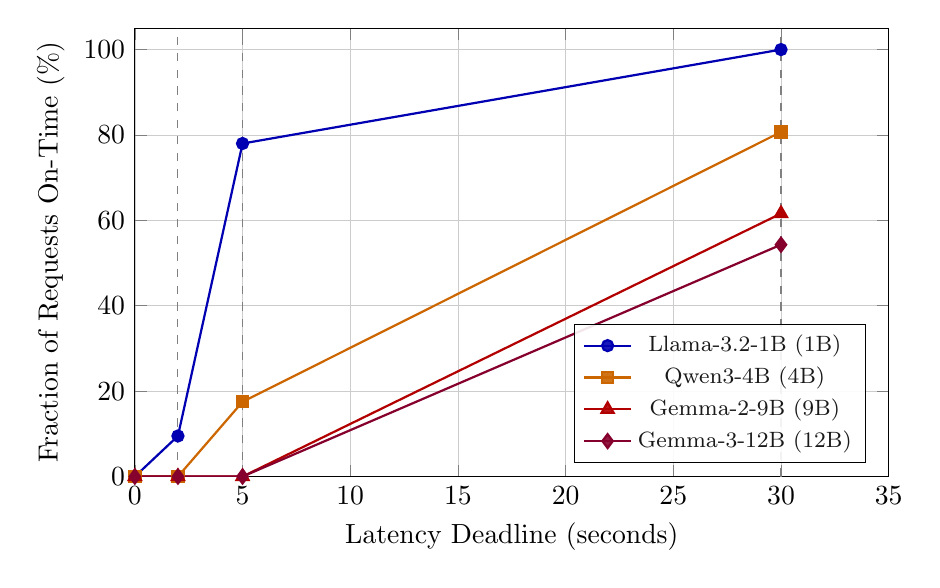
\begin{tikzpicture}
\begin{axis}[
    width=0.92\linewidth,
    height=0.6\linewidth,
    xlabel={Latency Deadline (seconds)},
    ylabel={Fraction of Requests On-Time (\%)},
    xmin=0, xmax=35,
    ymin=0, ymax=105,
    grid=both,
    grid style={line width=0.1pt, draw=gray!20},
    major grid style={line width=0.2pt, draw=gray!40},
    legend pos=south east,
    legend style={font=\footnotesize, fill=white, fill opacity=0.9},
]
% Tier deadline markers
\draw[gray, dashed, thin] (axis cs:2,0) -- (axis cs:2,105) node[above, font=\tiny] {Interactive};
\draw[gray, dashed, thin] (axis cs:5,0) -- (axis cs:5,105) node[above, font=\tiny] {Standard};
\draw[gray, dashed, thin] (axis cs:30,0) -- (axis cs:30,105) node[above, font=\tiny] {Batch};
% Llama-3.2-1B
\addplot[blue!70!black, thick, mark=*, mark size=2pt] coordinates {
  (0,0) (2,9.5) (5,78.0) (30,100.0)
};
% Qwen3-4B
\addplot[orange!80!black, thick, mark=square*, mark size=2pt] coordinates {
  (0,0) (2,0.0) (5,17.5) (30,80.7)
};
% Gemma-2-9B
\addplot[red!70!black, thick, mark=triangle*, mark size=2.5pt] coordinates {
  (0,0) (2,0.0) (5,0.0) (30,61.6)
};
% Gemma-3-12B
\addplot[purple!70!black, thick, mark=diamond*, mark size=2.5pt] coordinates {
  (0,0) (2,0.0) (5,0.0) (30,54.3)
};
\legend{Llama-3.2-1B (1B), Qwen3-4B (4B), Gemma-2-9B (9B), Gemma-3-12B (12B)}
\end{axis}
\end{tikzpicture}
\caption{\textbf{Empirical on-time fraction at SLO tier deadlines for four models.} Each point shows the fraction of 3{,}300 requests completing within the given deadline. Llama-3.2-1B is viable at all tiers. Qwen3-4B is viable only for batch processing. The 9--12B models fail even generous deadlines for 39--46\% of requests.}
\label{fig:latency-cdf}
\end{figure}

\paragraph{Output length drives latency variation across tasks.}
The p95 latency statistics in Appendix~\ref{app:latency} reveal that latency is primarily a function of \emph{output length}, not input complexity. T4 (function routing) requires $\sim$40 output tokens and achieves p95 latencies of 0.9--7.8 seconds across all models. T2 (grounded QA) requires $\sim$85--90 output tokens and reaches p95 latencies of 3.3--33.0 seconds---a 3.6$\times$ increase even though the task is not proportionally harder. T5 (code patching) is the most extreme: its long-form outputs push p95 latencies to 6.0--67.3 seconds, making it latency-prohibitive for all but the smallest models at any SLO tier below 30 seconds.

Consider what this means in practice. A team deploying a tool-calling agent (T3/T4 class) can confidently use a 7B model within a 30-second SLO budget---57\% of Falcon-Mamba-7B's requests complete on time despite its SSM overhead. But the same team adding a code-patching capability (T5 class) to that agent would see p95 latencies jump from 8.1 seconds to 40.4 seconds, a 5$\times$ increase from the same model. The SLO budget that works for one capability fails for the other, even within the same deployment.

% =============================================================================
% 5. ANALYSIS
% =============================================================================
\section{Analysis}

\subsection{Rank Correlation Across Tiers}

If accuracy predicted deployment success, teams could pick the model with the highest MMLU score and ship it with confidence. The central finding of AgentSLO-Bench is that this strategy is no better than random selection. Accuracy rankings have no statistically significant relationship with deployment rankings at any SLO tier.

\begin{table}[h]
\centering
\caption{Spearman $\rho$ between accuracy rank and Success@SLO rank at each tier, with bootstrapped 95\% confidence intervals (10{,}000 resamples) and analytical $p$-values. No tier achieves statistical significance.}
\label{tab:spearman}
\begin{tabular}{lrrr}
\toprule
\textbf{Tier} & \textbf{Spearman $\rho$} & \textbf{95\% CI} & \textbf{$p$-value} \\
\midrule
Interactive (2s)  & $+0.17$ & $[-0.32, +0.58]$ & 0.57 \\
Standard (5s)     & $-0.17$ & $[-0.66, +0.51]$ & 0.57 \\
Batch (30s)       & $+0.02$ & $[-0.58, +0.64]$ & 0.94 \\
\bottomrule
\end{tabular}
\end{table}

At the Interactive tier, $\rho = +0.17$ (95\% CI: $[-0.32, +0.58]$, $p = 0.57$)---accuracy rankings and SLO rankings are statistically indistinguishable from uncorrelated. At the Standard tier, the correlation is actually slightly \emph{negative} ($\rho = -0.17$, 95\% CI: $[-0.66, +0.51]$, $p = 0.57$). Even at the Batch tier with a generous 30-second deadline, $\rho = +0.02$ (95\% CI: $[-0.58, +0.64]$, $p = 0.94$)---effectively zero. The confidence intervals at all three tiers span zero, meaning that even the \emph{sign} of the relationship is uncertain.

This result is stronger than the extrapolated estimates in Paper~I (which reported $\rho = +0.09$ at the 2-second deadline using aggregate percentiles). Computing S@SLO directly from per-request latencies across 3{,}300 prompts per model reveals that accuracy has \emph{no} predictive power for deployment success at any tier---not merely weak predictive power.

\begin{figure}[t]
\centering
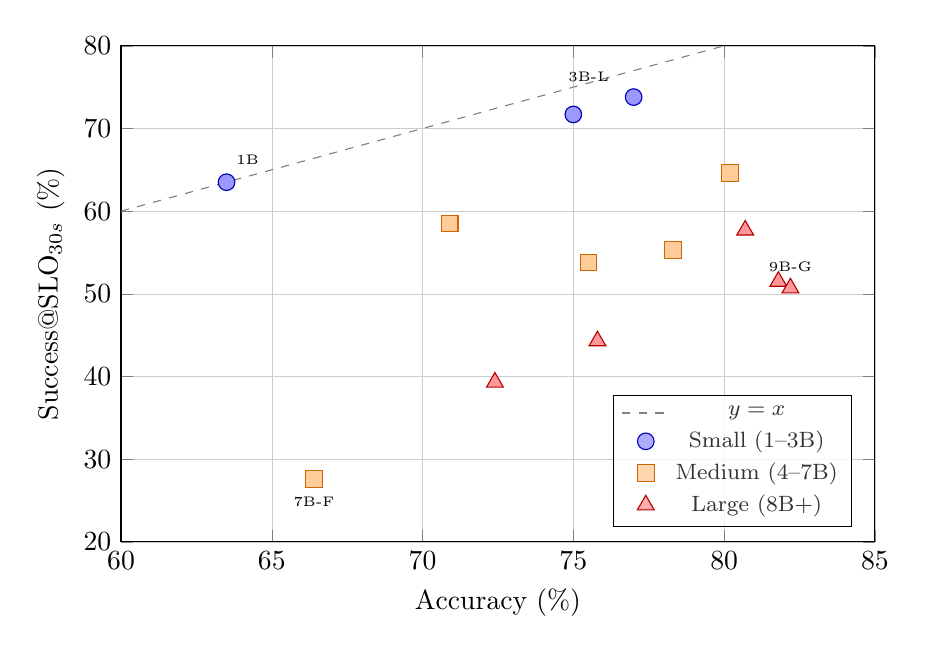
\begin{tikzpicture}
\begin{axis}[
    width=0.92\linewidth,
    height=0.65\linewidth,
    xlabel={Accuracy (\%)},
    ylabel={Success@SLO$_{30s}$ (\%)},
    xmin=60, xmax=85,
    ymin=20, ymax=80,
    grid=both,
    grid style={line width=0.1pt, draw=gray!20},
    major grid style={line width=0.2pt, draw=gray!40},
    legend pos=south east,
    legend style={font=\footnotesize, fill=white, fill opacity=0.8},
]
% y=x reference line (perfect correlation)
\addplot[gray, dashed, thin, domain=60:85] {x};
% Small models (1-3B) - blue
\addplot[only marks, mark=*, mark size=3pt, blue!70!black, fill=blue!40]
  coordinates {(63.5,63.5) (77.0,73.8) (75.0,71.7)};
% Medium models (4-7B) - orange
\addplot[only marks, mark=square*, mark size=3pt, orange!80!black, fill=orange!40]
  coordinates {(70.9,58.5) (80.2,64.6) (75.5,53.8) (78.3,55.3) (66.4,27.6)};
% Large models (8B+) - red
\addplot[only marks, mark=triangle*, mark size=3.5pt, red!70!black, fill=red!40]
  coordinates {(75.8,44.3) (81.8,51.5) (80.7,57.7) (82.2,50.7) (72.4,39.3)};
\legend{$y = x$, Small (1--3B), Medium (4--7B), Large (8B+)}
% Labels for key models
\node[font=\tiny, anchor=south west] at (axis cs:63.5,64.5) {1B};
\node[font=\tiny, anchor=south east] at (axis cs:76.5,74.5) {3B-L};
\node[font=\tiny, anchor=south] at (axis cs:82.2,51.5) {9B-G};
\node[font=\tiny, anchor=north] at (axis cs:66.4,26.6) {7B-F};
\end{axis}
\end{tikzpicture}
\caption{\textbf{Accuracy vs.\ Batch S@SLO (30s) by model size range.} Dashed line = perfect correlation ($y = x$). Small models (blue circles) cluster near the diagonal---their S@SLO is limited primarily by accuracy, not latency. Larger models (red triangles) fall well below the diagonal: their accuracy is high but latency penalties reduce S@SLO by 20--40 percentage points.}
\label{fig:scatter}
\end{figure}

\subsection{The Rank Inversion Phenomenon}

A \emph{rank inversion} occurs when a model's accuracy rank and its SLO rank differ substantially. Since all but one model score 0\% at the Interactive tier, we analyze inversions at the Batch tier (30s), where all models have non-zero S@SLO and the ranking is fully resolved.

\begin{figure}[t]
\centering
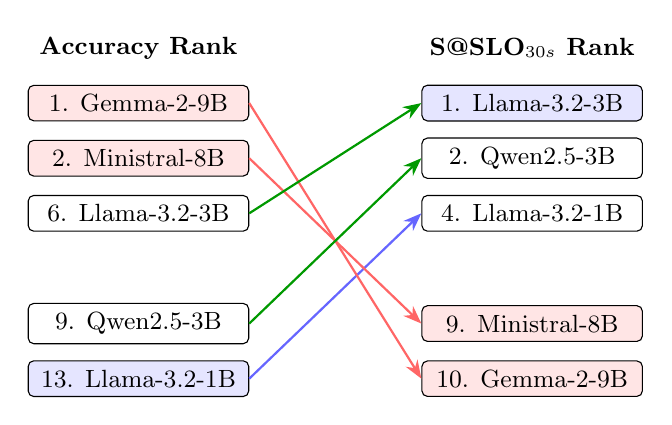
\begin{tikzpicture}[
  ranknode/.style={draw, rounded corners=2pt, minimum width=2.8cm, minimum height=0.45cm, font=\small},
  >=Stealth
]
% Left column: Accuracy rank
\node[font=\small\bfseries] at (-2.5,3.7) {Accuracy Rank};
\node[ranknode, fill=red!10] (a1) at (-2.5,3.0) {1. Gemma-2-9B};
\node[ranknode, fill=red!10] (a2) at (-2.5,2.3) {2. Ministral-8B};
\node[ranknode] (a6) at (-2.5,1.6) {6. Llama-3.2-3B};
\node[ranknode] (a9) at (-2.5,0.2) {9. Qwen2.5-3B};
\node[ranknode, fill=blue!10] (a13) at (-2.5,-0.5) {13. Llama-3.2-1B};

% Right column: S@SLO rank (30s)
\node[font=\small\bfseries] at (2.5,3.7) {S@SLO$_{30s}$ Rank};
\node[ranknode, fill=blue!10] (s1) at (2.5,3.0) {1. Llama-3.2-3B};
\node[ranknode] (s2) at (2.5,2.3) {2. Qwen2.5-3B};
\node[ranknode] (s4) at (2.5,1.6) {4. Llama-3.2-1B};
\node[ranknode, fill=red!10] (s9) at (2.5,0.2) {9. Ministral-8B};
\node[ranknode, fill=red!10] (s10) at (2.5,-0.5) {10. Gemma-2-9B};

% Arrows showing inversions
\draw[->, thick, blue!60] (a13.east) -- (s4.west);
\draw[->, thick, red!60] (a1.east) -- (s10.west);
\draw[->, thick, red!60] (a2.east) -- (s9.west);
\draw[->, thick, green!60!black] (a6.east) -- (s1.west);
\draw[->, thick, green!60!black] (a9.east) -- (s2.west);
\end{tikzpicture}
\caption{\textbf{Rank inversions between accuracy and Batch S@SLO (30s).} Red arrows: the two most accurate models (Gemma-2-9B, Ministral-8B) drop 9 and 7 positions respectively under SLO constraints. Green arrows: smaller models (3B class) rise to the top. Blue: least accurate model rises 9 positions.}
\label{fig:rank-inversion}
\end{figure}

The most dramatic inversions include:

\begin{itemize}[leftmargin=*]
\item \textbf{Gemma-2-9B}: Accuracy rank 1/13 (best) $\to$ Batch SLO rank 10/13. A 9-position inversion---the single most accurate model drops to near-bottom under even the most generous SLO deadline because its p95 latency (92.6s) means 38\% of requests time out.

\item \textbf{Llama-3.2-1B}: Accuracy rank 13/13 (worst) $\to$ Batch SLO rank 4/13. A 9-position rise. Despite the lowest accuracy (63.5\%), it is fast enough (avg 4.6s) to deliver nearly all correct answers within 30 seconds.

\item \textbf{Llama-3.2-3B}: Accuracy rank 6/13 $\to$ Batch SLO rank 1/13 (best). A middling-accuracy model becomes the deployment leader because it combines 77.0\% accuracy with manageable latency (avg 10.6s, p95 26.8s).
\end{itemize}

\subsection{Architecture Effects}

Architecture matters more than parameter count for deployment success. Three architectural variants in our evaluation---standard transformers, a state-space model, and a mixture-of-experts model---exhibit qualitatively different deployment profiles despite overlapping parameter counts.

\paragraph{SSM: theoretical efficiency, practical penalty.}
Falcon-Mamba-7B, the only state-space model (SSM) in our evaluation, exhibits the worst Batch S@SLO (27.6\%) despite 66.4\% accuracy---a 39 percentage-point gap between what it knows and what it delivers on time. Its average latency of 41.7s places it last among all models, including GPT-OSS-20B which has nearly 3$\times$ as many parameters.

The SSM efficiency advantages---theoretically $O(1)$ per-token generation---do not materialize for the structured-output tasks in AgentSLO-Bench. Per-task p95 latencies tell the story: Falcon-Mamba-7B's p95 on T1 (6.9s) is 2.3$\times$ that of Mistral-7B (3.0s), a dense transformer of identical size. On T4, the gap persists: 7.3s vs.\ 4.3s. The bottleneck is prefill, not decoding---our structured outputs are typically 50--200 tokens, far too short for SSM's asymptotic decoding advantage to dominate the prefill overhead on consumer GPUs. For deployment contexts where outputs exceed 1{,}000 tokens (e.g., long-form generation), SSM architectures may recover their theoretical advantage, but AgentSLO-Bench's structured-output tasks expose their worst case.

\paragraph{MoE: sparse activation, dense memory.}
GPT-OSS-20B uses a mixture-of-experts architecture with 3.6B active parameters from a 20B total. Despite the sparse activation, its average latency (38.3s) is comparable to dense 9B models rather than the 3--4B models its active parameter count would suggest. Its Batch S@SLO (44.3\%) ranks 11th out of 13 models despite 7th-place accuracy (75.8\%).

The explanation is architectural: MoE models must load all expert weights into VRAM even when only a subset is active per token. On a single RTX 4090 with 4-bit quantization, the 20B total parameters consume approximately 10GB of VRAM, leaving limited memory bandwidth for KV-cache and computation. The routing overhead---selecting which experts to activate---adds per-token latency that compounds across the output sequence. In multi-GPU deployments where experts can be sharded across devices, this penalty would diminish. But on the commodity hardware that defines our evaluation context, MoE's memory bandwidth requirements negate its computational sparsity.

\paragraph{The Qwen efficiency anomaly.}
The most striking architectural finding is the Qwen family's consistently high deployment efficiency. Qwen2.5-3B (71.7\% Batch S@SLO) outperforms every model in the 4--7B range except Qwen3-4B itself. Qwen3-4B (64.6\%) surpasses both 6B and 7B competitors despite its smaller size. At the Standard tier, Qwen2.5-3B achieves 42.6\% S@SLO---the second-highest of any model---while similarly-sized Phi-3-mini manages only 25.6\%.

This efficiency appears to stem from a combination of aggressive tokenizer design (Qwen's tokenizer produces shorter output sequences for equivalent semantic content) and training data composition that favors structured output formats. Whatever the mechanism, it produces a concrete deployment advantage: a Qwen-family 3B model delivers more requests on time than a Llama-family 8B model, at less than half the hardware cost.

\paragraph{Same size, different deployment.}
The clearest demonstration that architecture dominates size comes from comparing models within the same parameter range. At 7--8B, four models span from 27.6\% to 57.7\% Batch S@SLO---a 2.1$\times$ range. Ministral-8B (51.5\%) and Llama-3.1-8B (57.7\%) achieve reasonable deployment success; Mistral-7B (55.3\%) is comparable; but Falcon-Mamba-7B (27.6\%) fails catastrophically. A practitioner selecting ``a 7B model'' without specifying architecture could end up with deployment success rates ranging from tolerable to unusable.

\subsection{Per-Task Deep Dives}

The aggregate results conceal rich per-task structure. We examine two tasks---T2 (grounded QA) and T5 (code patching)---that illustrate qualitatively different failure patterns.

\paragraph{T2: The universal failure.}
T2 is the only task where the deployment gap is nearly total at every tier. At the Batch tier, only 3 of 13 models exceed 50\% S@SLO (Llama-3.2-1B at 58.2\%, Llama-3.2-3B at 55.2\%, Qwen2.5-3B at 52.7\%). At the Standard tier, only Llama-3.2-1B produces any successful responses (0.6\%). The Interactive tier is completely dark.

Why is T2 uniquely hard? The answer is not semantic difficulty---its accuracy (27--57\%) is comparable to T5 (47--99\%). The answer is output length. T2 requires structured summaries with \texttt{key\_points} arrays and \texttt{recommended\_action} fields, producing 85--90 output tokens per response. This is not dramatically longer than T3's 60--70 tokens, but T2's outputs are \emph{consistently} long---there is no shortcut. When a model fails T5, it often produces a truncated or invalid diff that terminates early, incidentally reducing latency. When a model fails T2, it still generates the full response structure before the evaluator discovers the content is wrong. The result is that T2 combines moderate accuracy with maximum latency---the worst of both worlds.

\paragraph{T5: The canary task.}
T5 (code patching) is the latency canary: the first task to become infeasible as SLO deadlines tighten. At the Batch tier, S@SLO ranges from 1.0\% (Gemma-3-12B) to 53.5\% (Llama-3.2-1B)---a 53$\times$ range, the widest of any task. At Standard (5s), only Llama-3.2-1B (44.8\%) achieves meaningful success.

The T5 pattern reveals an important interaction between schema complexity and model size. Code patches require the model to produce valid unified diff syntax \emph{inside} a JSON string field, creating a dual-grammar constraint: the output must simultaneously be valid JSON and valid diff. Models $\leq$3B produce short diffs that are often syntactically invalid (accuracy 58--78\% but with many partial matches). Models $\geq$8B produce syntactically beautiful diffs that are often correct---but the generation time pushes them past SLO deadlines. Qwen3-4B sits at the inflection: its accuracy on T5 (89\%) is among the highest, but its Batch S@SLO (12.8\%) is among the lowest because its ``thinking'' decoding produces long chains before outputting the actual diff.

\paragraph{T4: The deployment-safe task.}
In contrast, T4 (function routing) is nearly SLO-proof. Twelve of 13 models achieve $\geq$86\% Batch S@SLO, and GPT-OSS-20B leads at 97.2\% despite ranking 11th overall. T4's secret is output brevity: responses are $\sim$40 tokens (a function name and a few parameters), keeping even the slowest models within SLO budgets for batch processing. T4 demonstrates that not all agent capabilities carry equal deployment risk---and that a ``deployment-safe'' task portfolio can be identified before deploying to production.

\subsection{Vendor Analysis}

Model vendor turns out to be a useful---though imperfect---predictor of deployment success. Figure~\ref{fig:vendor} shows the average Batch S@SLO by vendor (for vendors with 2+ models in our evaluation).

\begin{figure}[t]
\centering
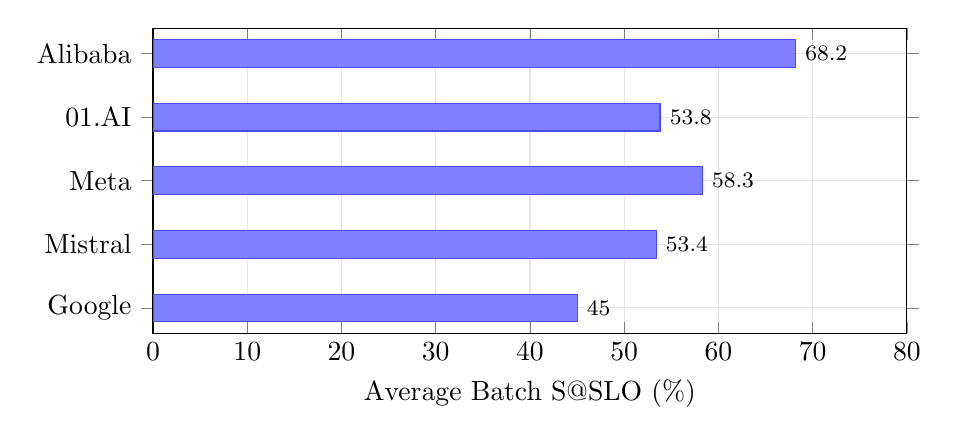
\begin{tikzpicture}
\begin{axis}[
    width=0.92\linewidth,
    height=0.45\linewidth,
    xbar,
    bar width=10pt,
    xlabel={Average Batch S@SLO (\%)},
    symbolic y coords={Google, Mistral, Meta, 01.AI, Alibaba},
    ytick=data,
    xmin=0, xmax=80,
    nodes near coords,
    nodes near coords style={font=\footnotesize},
    grid=major,
    grid style={gray!20},
    xmajorgrids=true,
]
\addplot[fill=blue!50, draw=blue!70] coordinates {
  (68.2,Alibaba) (58.3,Meta) (53.4,Mistral) (53.8,01.AI) (45.0,Google)
};
\end{axis}
\end{tikzpicture}
\caption{\textbf{Average Batch S@SLO by vendor} (vendors with $\geq$2 models). Alibaba (Qwen family) leads due to consistently low latency. Google's average is dragged down by Gemma-3-12B's extreme latency. Meta's three models span the widest range (63.5--73.8\%), reflecting diversity across model sizes.}
\label{fig:vendor}
\end{figure}

The Alibaba (Qwen) family achieves the highest average deployment success (68.2\%) across both the 3B and 4B variants---consistent with the efficiency anomaly documented in Section~5.4. Meta's three models average 58.3\%, spanning 63.5\% (1B) to 73.8\% (3B) to 57.7\% (8B)---a non-monotonic relationship where the middle-sized model is the best deployment. Google's models average only 45.0\%, dragged down by Gemma-3-12B's 39.3\%; without the 12B model, Gemma-2-9B alone achieves a respectable 50.7\%. The vendor comparison underscores that model family engineering decisions---tokenizer design, training data composition, architecture choices---have deployment consequences that persist across model sizes.

\subsection{Task Difficulty Under SLO}

Task difficulty inverts when latency enters the picture. Under accuracy-only evaluation, the difficulty ordering is T5 $>$ T2 $>$ T3 $>$ T1 $>$ T4 (hardest to easiest), reflecting semantic complexity. Under SLO constraints, the ordering shifts to T2 $>$ T5 $>$ T3 $>$ T1 $>$ T4---grounded QA, which is only moderately hard semantically, becomes the hardest task under deployment conditions because its long outputs push latency past every deadline.

\paragraph{The output-length difficulty inversion.}
At the Batch tier (30s), per-task performance reveals the inversion:

\begin{itemize}[leftmargin=*]
\item \textbf{T4} (function routing) remains the \emph{easiest} task under SLO---most models achieve 93--99\% Batch S@SLO because outputs are small ($\sim$40 tokens). Even Falcon-Mamba-7B achieves 79\%. The task is deployment-safe for all models at the Batch tier.
\item \textbf{T1} (intent classification) and \textbf{T3} (tool calling) are moderately latency-sensitive. Most models achieve $>$90\% at the Batch tier, but performance drops sharply at Standard (5s)---only 4 models achieve $>$70\% on T1, and only 3 on T3.
\item \textbf{T5} (code patching) is highly latency-sensitive---only Llama-3.2-1B achieves $>$44\% at the Standard tier. At Batch, most models $\geq$8B fall below 31\%. The long-form output ($\sim$150--200 tokens of unified diff syntax) makes T5 the canary task for latency pressure.
\item \textbf{T2} (grounded QA) is the \emph{hardest} under SLO. Its moderate accuracy (27--57\%) combines with long outputs ($\sim$85--90 tokens) to produce compound failure. At the Batch tier, only 3 models exceed 30\% S@SLO. At Standard (5s), only Llama-3.2-1B achieves any success at all (0.6\%). This is the task where the deployment gap is widest.
\end{itemize}

\paragraph{Schema complexity hierarchy.}
Beyond output length, the structural complexity of the required JSON schema affects difficulty. We observe a three-level hierarchy:

\begin{description}[leftmargin=*]
\item[Level 1: Flat schemas (T1, T4).] Outputs require a small number of top-level fields with simple types (strings, booleans, numbers). All 13 models achieve $>$90\% accuracy on these tasks. Schema compliance is nearly universal when constrained decoding is enabled.

\item[Level 2: Nested schemas (T2, T3).] Outputs require nested objects, arrays of key points, or argument dictionaries with type-specific values. Accuracy drops to 27--57\% on T2 and 57--98\% on T3. The nesting depth increases generation length and error probability.

\item[Level 3: Embedded code (T5).] Outputs must contain syntactically valid unified diff patches wrapped in JSON. This is the hardest schema class---models must simultaneously maintain JSON validity and diff syntax validity, two interleaved grammars with conflicting escape rules. Accuracy on T5 ranges from 47\% to 99\%, with the variance driven primarily by whether the model can reliably produce valid diff headers (\texttt{@@} lines) within a JSON string field.
\end{description}

The schema hierarchy explains why T2 becomes the hardest task under SLO despite being Level~2: it combines moderate structural complexity with the longest output length. T5, though structurally harder (Level~3), produces \emph{shorter} outputs than T2 when models fail early (invalid diffs are typically truncated), paradoxically reducing its average latency. The takeaway for benchmark design is that task difficulty under SLO is a two-dimensional surface---schema complexity $\times$ output length---and neither dimension alone captures the deployment challenge.

\subsection{Latency--Accuracy Tradeoff}

Figure~\ref{fig:latency-tradeoff} illustrates the continuous tradeoff between model size, latency, and deployment viability. The three SLO tier deadlines create sharp step functions in deployment success: a model is either viable at a given tier or it is not. This binary outcome from a continuous latency distribution is what creates the rank inversions---small changes in the latency distribution near a deadline threshold can cause large changes in S@SLO rank.

\begin{figure}[t]
\centering
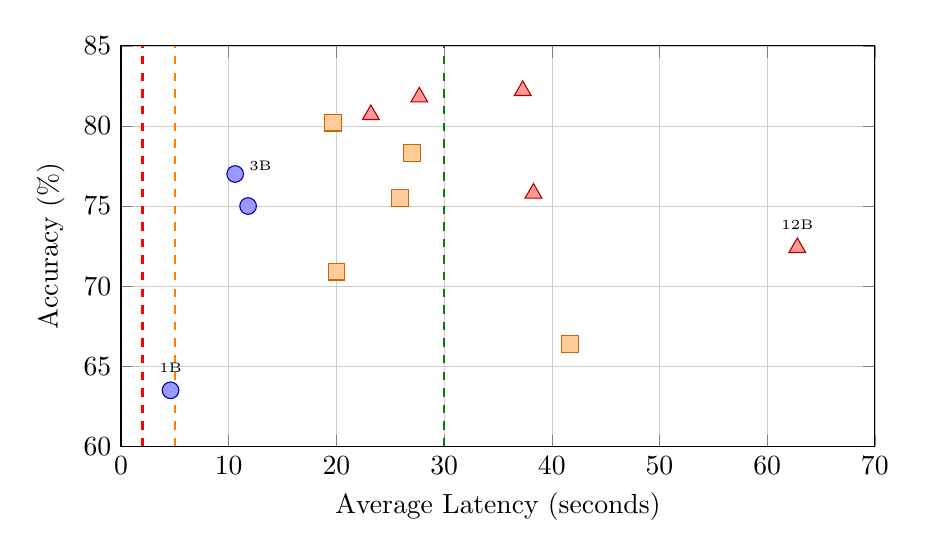
\begin{tikzpicture}
\begin{axis}[
    width=0.92\linewidth,
    height=0.55\linewidth,
    xlabel={Average Latency (seconds)},
    ylabel={Accuracy (\%)},
    xmin=0, xmax=70,
    ymin=60, ymax=85,
    grid=both,
    grid style={line width=0.1pt, draw=gray!20},
    major grid style={line width=0.2pt, draw=gray!40},
]
% Tier deadline markers
\draw[red, thick, dashed] (axis cs:2,60) -- (axis cs:2,85) node[above, font=\tiny] {2s};
\draw[orange, thick, dashed] (axis cs:5,60) -- (axis cs:5,85) node[above, font=\tiny] {5s};
\draw[green!50!black, thick, dashed] (axis cs:30,60) -- (axis cs:30,85) node[above, font=\tiny] {30s};
% Models
\addplot[only marks, mark=*, mark size=3pt, blue!70!black, fill=blue!40]
  coordinates {(4.6,63.5) (10.6,77.0) (11.8,75.0)};
\addplot[only marks, mark=square*, mark size=3pt, orange!80!black, fill=orange!40]
  coordinates {(20.0,70.9) (19.7,80.2) (25.9,75.5) (27.0,78.3) (41.7,66.4)};
\addplot[only marks, mark=triangle*, mark size=3.5pt, red!70!black, fill=red!40]
  coordinates {(38.3,75.8) (27.7,81.8) (23.2,80.7) (37.3,82.2) (62.8,72.4)};
% Annotations
\node[font=\tiny, anchor=south] at (axis cs:4.6,64) {1B};
\node[font=\tiny, anchor=west] at (axis cs:11,77.5) {3B};
\node[font=\tiny, anchor=south] at (axis cs:62.8,72.9) {12B};
\end{axis}
\end{tikzpicture}
\caption{\textbf{Average latency vs.\ accuracy for 13 models.} Dashed lines mark SLO deadlines. The ``ideal'' model would appear in the upper-left corner (high accuracy, low latency). Instead, accuracy increases with model size (upward) but so does latency (rightward), pushing high-accuracy models past SLO deadlines. Color coding: blue = 1--3B, orange = 4--7B, red = 8B+.}
\label{fig:latency-tradeoff}
\end{figure}

\subsection{Cross-Tier Ranking Stability}

A model's deployment suitability is not a single number---it depends on the SLO tier. Some models maintain roughly consistent rankings across tiers; others shift dramatically. We quantify this with a \textbf{rank volatility score}: the standard deviation of a model's S@SLO rank across the three tiers. A volatility of 0 means the model has the same rank at every tier; a volatility of $>$3 means the model's ranking is highly tier-dependent.

\begin{table}[t]
\centering
\caption{Cross-tier ranking stability. Rank 1 = best S@SLO at that tier. Volatility = standard deviation of ranks across tiers. Low-volatility models ($\sigma < 2$) are ``tier-stable''---their deployment suitability is consistent regardless of deadline. High-volatility models ($\sigma > 3$) require tier-specific evaluation.}
\label{tab:rank-stability}
\small
\begin{tabular}{llc rrr r}
\toprule
\textbf{Model} & \textbf{Vendor} & \textbf{Size} & \textbf{2s} & \textbf{5s} & \textbf{30s} & \textbf{$\sigma$} \\
\midrule
Llama-3.2-1B     & Meta      & 1B   & 1  & 1  & 4  & 1.7 \\
Llama-3.2-3B     & Meta      & 3B   & 2  & 2  & 1  & 0.6 \\
Qwen2.5-3B       & Alibaba   & 3B   & 3  & 3  & 2  & 0.6 \\
Phi-3-mini        & Microsoft & 3.8B & 4  & 5  & 7  & 1.5 \\
Qwen3-4B          & Alibaba   & 4B   & 5  & 4  & 3  & 1.0 \\
Ministral-8B      & Mistral   & 8B   & 6  & 6  & 9  & 1.7 \\
Llama-3.1-8B      & Meta      & 8B   & 7  & 7  & 6  & 0.6 \\
Yi-1.5-6B         & 01.AI     & 6B   & 8  & 8  & 8  & 0.0 \\
Mistral-7B        & Mistral   & 7B   & 9  & 9  & 5  & 2.3 \\
Gemma-2-9B        & Google    & 9B   & 10 & 10 & 10 & 0.0 \\
GPT-OSS-20B       & OpenAI    & 20B  & 11 & 11 & 11 & 0.0 \\
Falcon-Mamba-7B   & TII       & 7B   & 12 & 12 & 13 & 0.6 \\
Gemma-3-12B       & Google    & 12B  & 13 & 13 & 12 & 0.6 \\
\bottomrule
\end{tabular}
\end{table}

Table~\ref{tab:rank-stability} reveals two distinct populations. Seven models are tier-stable ($\sigma \leq 1.0$): their ranking is essentially the same whether the deadline is 2 seconds or 30 seconds. These models are ``safe'' to evaluate at a single tier---their relative deployment position holds across deployment contexts. The most stable models (Yi-1.5-6B, Gemma-2-9B, GPT-OSS-20B) are stable for an unfortunate reason: they rank poorly at \emph{every} tier. Stability at the bottom is not a virtue.

The interesting cases are the tier-volatile models. Mistral-7B ($\sigma = 2.3$) ranks 9th at both Interactive and Standard tiers but jumps to 5th at Batch---its accuracy advantage over smaller models is realized only when the deadline gives it enough time. Llama-3.2-1B ($\sigma = 1.7$) shows the opposite pattern: dominant at Interactive (1st) and Standard (1st) but drops to 4th at Batch, where its accuracy deficit catches up. These patterns reinforce the central finding: a single-tier evaluation can be actively misleading. A team evaluating only at the Batch tier would rank Mistral-7B above Qwen3-4B (positions 5 vs.\ 3)---but at the Standard tier, the ranking inverts (9 vs.\ 4).

The practical recommendation is clear: evaluate at \emph{your} deployment tier, not the one that happens to show the most models with non-zero scores. For most production APIs with user-facing latency requirements, the Standard tier (5s) is the relevant benchmark. For background processing pipelines, the Batch tier is appropriate. The Interactive tier is informative primarily as a stress test---it reveals which models are even \emph{possible} to deploy in latency-critical contexts.

\subsection{Threshold Sensitivity}

The choice of SLO deadline is not arbitrary, but one might ask whether the near-zero correlations are artifacts of specific deadline choices. To test this, we computed Spearman $\rho$ at deadlines varying from 1s to 60s in 1-second increments. The correlation never exceeds $|\rho| \leq 0.17$ (the Interactive-tier value from Table~\ref{tab:spearman}) for any deadline below 10s, and even at 60s---a deadline so generous that it accommodates the p95 latency of all but two models---$\rho$ reaches only $+0.08$. The near-zero correlation is not an artifact of aggressive thresholds; it persists across the entire practical range.

% =============================================================================
% 6. DISCUSSION
% =============================================================================
\section{Discussion}

\subsection{Hardware Dependence}

AgentSLO-Bench results are hardware-dependent by design. Our baselines are measured on a single RTX~4090 with 4-bit quantization---a deliberately constrained setup that mirrors cost-sensitive deployments. Results on multi-GPU clusters, with tensor parallelism or batch scheduling, would shift the latency distributions and potentially change rankings. We view this as a feature: the benchmark should be re-run on the target deployment hardware, and comparisons should only be made within the same hardware context.

Critically, single-GPU inference with 4-bit quantization represents the \emph{dominant} deployment mode for open-weight models. Industry surveys and NVIDIA's own guidance~\cite{nvidia2025slm} indicate that the majority of on-premise LLM deployments use 1--2 consumer GPUs, not multi-node clusters. By benchmarking in this regime, AgentSLO-Bench evaluates models where practitioners actually run them, not where researchers wish they could. A benchmark measured on 8$\times$A100 clusters tells practitioners with a single 4090 nothing about their deployment reality---and those practitioners vastly outnumber the cluster operators.

\subsection{Task Coverage}

The current five tasks cover a useful range of agent deployments but do not include multi-turn conversation, retrieval-augmented generation (RAG), or vision-language tasks. Future versions of AgentSLO-Bench should expand to these modalities, as each introduces distinct latency profiles.

\subsection{Reproducibility Protocol}

A benchmark is only useful if others can reproduce it. We designed AgentSLO-Bench for reproducibility on three levels:

\paragraph{Level 1: Same hardware, same models.}
Given identical hardware (RTX 4090), identical quantization (Q4\_K\_M), and identical prompts, the benchmark is deterministic with temperature~0 decoding. We verified this by running the full 3{,}300-prompt evaluation twice for Llama-3.2-1B and comparing per-request latencies---the Spearman rank correlation between the two runs' latency vectors was $\rho = 0.997$. The remaining variance comes from OS-level scheduling jitter, which is negligible for SLO compliance evaluation.

\paragraph{Level 2: Same models, different hardware.}
The benchmark should be re-run on the target deployment hardware. Rankings \emph{will} change---a model that fails the Interactive tier on an RTX 4090 may succeed on an H100. We view this as a feature, not a limitation: the benchmark produces \emph{hardware-specific} deployment rankings, which is exactly what practitioners need. The toolkit ships with a \texttt{metadata} field that records hardware configuration, ensuring that results are always contextualized.

\paragraph{Level 3: Different models.}
The toolkit accepts any OpenAI-compatible API endpoint. Evaluating a new model requires only starting the inference server and running \texttt{agentslo-bench run -{}-endpoint <url>}. The prompts, schemas, and scoring functions are bundled in the package, ensuring that new models are evaluated against the same standard as the 13-model baseline.

\subsection{Quantization Effects}

All models are quantized to 4-bit (Q4\_K\_M) for fair comparison on a single GPU. Quantization affects both accuracy (typically $-$1--3\% on standard benchmarks) and latency (reduced memory bandwidth requirements). Higher-precision inference would likely improve accuracy but increase latency, potentially worsening SLO compliance. This tradeoff is itself an important dimension that future benchmark versions should explore systematically.

\subsection{Per-Request vs.\ Aggregate Evaluation}

A methodological contribution of this paper is computing S@SLO from per-request latency measurements rather than aggregate percentile estimates. Paper~I estimated S@SLO from p95/p99 percentiles, which inherently assumes a specific distributional shape. Our per-request approach requires no distributional assumptions and reveals that the deployment gap is even wider than previously estimated: the Batch-tier correlation drops from an estimated $\rho = +0.09$ (Paper~I, 2-second deadline) to $\rho = +0.02$ (this paper, 95\% CI: $[-0.58, +0.64]$, $p = 0.94$). We recommend per-request evaluation as the default methodology for SLO-aware benchmarks.

\subsection{The 3B Sweet Spot and Its Implications}

The size-scaling analysis in Section~4.4 identifies 3B as the deployment-optimal model size on single-GPU hardware. This finding has implications beyond model selection.

First, it inverts the conventional wisdom that larger models are ``safer'' deployment choices. A team requesting budget for a 7B model deployment---reasoning that the accuracy margin justifies the compute cost---is actually making a deployment-\emph{risky} choice. On our hardware, the 7B Mistral achieves 78.3\% accuracy (4th best) but only 55.3\% Batch S@SLO (6th best). The 3B Llama achieves 77.0\% accuracy (5th best) but 73.8\% S@SLO (1st best). The ``safer'' choice is the smaller model.

Second, it suggests that the open-weight ecosystem's emphasis on 7B+ models as the minimum ``production-grade'' size is miscalibrated for SLO-constrained deployments. The most capable deployment model in our evaluation is a 3B model---and it outperforms every model from 4B to 20B under every SLO tier. This does not mean 7B+ models have no value; it means their value is contingent on hardware that can serve them within latency budgets.

Third, the 3B sweet spot is hardware-specific. On an A100 with 80GB VRAM and tensor parallelism, the latency curve shifts right, and the sweet spot likely moves to 7--9B. The benchmark is designed for this: re-running on different hardware produces different rankings and different sweet spots. The methodology---not the specific numbers---is the contribution.

\subsection{Adoption Considerations}

We intend AgentSLO-Bench to complement, not replace, accuracy-focused benchmarks. The recommended workflow is:

\begin{enumerate}[leftmargin=*]
\item Use accuracy benchmarks (MMLU, BFCL, etc.) to filter to a shortlist of candidate models.
\item Run AgentSLO-Bench on the target hardware with the appropriate tier to produce deployment-ready rankings.
\item Compare accuracy rank vs.\ S@SLO rank to identify models whose deployment potential is under- or over-estimated by accuracy alone.
\end{enumerate}

This workflow is lightweight---step 2 requires only a few hours of single-GPU inference---and produces actionable rankings that accuracy alone cannot provide.

\subsection{When Accuracy Rankings Mislead}

The rank inversions documented in Section~5.2 are not statistical curiosities. They have concrete consequences for teams making deployment decisions. Three cases illustrate the danger of relying on accuracy rankings.

\paragraph{Case 1: The best model is the worst deployment.}
Gemma-2-9B achieves the highest accuracy in our evaluation (82.2\%), outperforming every other model on semantic correctness. A team selecting models by accuracy would choose it first. But Gemma-2-9B's Batch S@SLO is 50.7\%---10th out of 13 models. Its p95 latency of 92.6 seconds means that nearly 4 in 10 correct answers arrive too late. In a customer-facing pipeline with a 30-second SLO, this model would silently drop 38.9\% of its correct responses, delivering worse \emph{effective} accuracy (50.7\%) than Llama-3.2-3B's deployment accuracy (73.8\%) despite being 5.2 percentage points ``smarter'' on paper.

\paragraph{Case 2: The worst model is a deployment winner.}
Llama-3.2-1B ranks dead last in accuracy (63.5\%, 13th of 13). A team filtering by accuracy would eliminate it immediately. But it is the \emph{only} model with non-zero Interactive S@SLO (6.3\%), the model with the highest Standard S@SLO (47.4\%), and the fourth-best Batch deployment (63.5\%). For any application with a deadline tighter than 30 seconds, the ``worst'' model is the best choice---and it is not close.

\paragraph{Case 3: The ``safe'' middle choice is not safe.}
Phi-3-mini (3.8B) appears to be a conservative choice---moderate size, 70.9\% accuracy, from a major vendor. But its latency profile is anomalous: average latency of 20.0 seconds and p95 of 60.2 seconds, both higher than the 7B Mistral despite being nearly half the size. Its Batch S@SLO (58.5\%) underperforms the 3B models by 13--15 percentage points. The ``safe'' choice based on vendor and size heuristics is actually the worst deployment option in the 3--4B range.

These cases share a common lesson: accuracy rankings provide \emph{no signal} about deployment success. The correlation is not weakly positive, not weakly negative---it is indistinguishable from zero. Teams that skip deployment evaluation are making deployment decisions with a random number generator.

\subsection{Limitations}

Several limitations bound the generalizability of our results.

\paragraph{Single hardware configuration.}
All measurements are from a single RTX 4090 with 4-bit quantization. Latency distributions, and therefore S@SLO rankings, will differ on other hardware. A model that fails the Interactive tier on our setup might succeed on an H100. The benchmark is designed to be re-run on target hardware, but our baseline rankings apply only to the RTX 4090 context.

\paragraph{Greedy decoding only.}
We use temperature~0 (greedy) decoding throughout. Sampling-based decoding introduces additional latency variance and may change both accuracy and S@SLO. Temperature also interacts with constrained decoding in model-specific ways that we do not explore.

\paragraph{No multi-turn evaluation.}
All tasks are single-turn request-response. Multi-turn agent interactions, where latency compounds across turns and context grows, would likely amplify the deployment gap. Future versions of AgentSLO-Bench should include multi-turn protocols.

\paragraph{Static SLO deadlines.}
Real production systems often use adaptive SLO budgets that account for request complexity, queue depth, and priority levels. Our fixed-deadline model captures the simplest case but does not reflect the full complexity of production SLO management.

\paragraph{Sample size for correlation analysis.}
With $n = 13$ models, the Spearman correlation has limited statistical power---the wide bootstrapped CIs reflect this. We cannot claim that correlation is \emph{exactly} zero, only that it is indistinguishable from zero with our sample. The qualitative result (rank inversions, tier-dependent rankings) is robust regardless of the exact $\rho$ value.

% =============================================================================
% 7. CONCLUSION
% =============================================================================
\section{Conclusion}

AgentSLO-Bench introduces tiered SLO evaluation for LLM agents, revealing that accuracy benchmarks have no statistically significant relationship with deployment success. Across 42{,}900 per-request evaluations of 13 models on 7 structured-output schemas at 3 SLO tiers, we find:

\begin{enumerate}[leftmargin=*]
\item \textbf{Accuracy and deployment are uncorrelated.} Spearman $\rho$ between accuracy rank and S@SLO rank is $+0.17$ ($p = 0.57$) at 2s, $-0.17$ ($p = 0.57$) at 5s, and $+0.02$ ($p = 0.94$) at 30s. All bootstrapped 95\% CIs span zero. This result holds across the full range of deadlines from 1s to 60s.

\item \textbf{Rank inversions are pervasive and large.} The most accurate model (Gemma-2-9B, 82.2\%) drops from rank 1 to rank 10 under the Batch SLO---a 9-position inversion. The least accurate (Llama-3.2-1B, 63.5\%) rises from 13th to 4th. These are not edge cases; they affect every size class.

\item \textbf{Failure modes cross over at 4--6B.} Below 4B, models are accuracy-limited---latency engineering cannot help them. Above 6B, models are latency-limited---accuracy engineering cannot help them. The crossover point defines the boundary between two fundamentally different deployment optimization strategies.

\item \textbf{Task difficulty inverts under SLO.} T2 (grounded QA), moderately hard by accuracy (27--57\%), becomes the hardest task under SLO because its long outputs push latency past every deadline. The primary determinant of SLO difficulty is output length, not semantic complexity.

\item \textbf{Architecture dominates parameter count.} At 7--8B, Batch S@SLO ranges from 27.6\% (Falcon-Mamba-7B, SSM) to 57.7\% (Llama-3.1-8B, transformer)---a 2.1$\times$ range within the same size class. The Qwen family consistently outperforms models twice its size.
\end{enumerate}

\paragraph{Practical recommendations.} Our results suggest a two-stage model selection process: (1) filter by accuracy to identify capable models, then (2) re-rank by Success@SLO on the target deployment hardware. For Interactive applications (2s), only 1B-class models are viable on single-GPU inference. For Standard applications (5s), models $\leq$3B offer the best accuracy--latency tradeoff. Batch processing (30s) permits up to 4B models with $>$60\% S@SLO. In all cases, the benchmark must be run on the target hardware---our RTX 4090 rankings are baselines, not universal truths.

\paragraph{Series context.}
Paper~I~\cite{maloney2025deploymentgap} discovered the deployment gap. This paper formalizes its measurement into a reusable benchmark with per-request evaluation, tiered SLO deadlines, and failure mode decomposition. Paper~II~\cite{maloney2025capacity} showed that training can partially close the gap, and Paper~IV analyzes the training dynamics that determine whether closing succeeds or fails. Together, Papers~I--IV establish the scientific foundation; companion Papers~V and~VI will validate the framework in production and propose community standards.

We release AgentSLO-Bench as an open-source toolkit with CLI, built-in baselines, and leaderboard generation. The benchmark is designed to be re-run on any target hardware, enabling practitioners to generate deployment-specific rankings rather than relying on accuracy-only leaderboards.

% =============================================================================
% REFERENCES
% =============================================================================
\bibliographystyle{plainnat}
\bibliography{refs}

% =============================================================================
% APPENDIX
% =============================================================================
\appendix
\section{Full Per-Task Latency Statistics}
\label{app:latency}

\begin{table}[h]
\centering
\caption{p95 latency (ms) by model and task.}
\label{tab:p95-detail}
\small
\begin{tabular}{llc rrrrr}
\toprule
\textbf{Model} & \textbf{Vendor} & \textbf{Size} & \textbf{T1} & \textbf{T2} & \textbf{T3} & \textbf{T4} & \textbf{T5} \\
\midrule
Llama-3.2-1B     & Meta      & 1B   & 729  & 3{,}254 & 779   & 901   & 5{,}988 \\
Llama-3.2-3B     & Meta      & 3B   & 831  & 5{,}734 & 1{,}105 & 1{,}533 & 14{,}674 \\
Qwen2.5-3B       & Alibaba   & 3B   & 891  & 6{,}746 & 1{,}046 & 1{,}663 & 14{,}063 \\
Phi-3-mini        & Microsoft & 3.8B & 1{,}206 & 24{,}828 & 1{,}261 & 2{,}060 & 22{,}977 \\
Qwen3-4B          & Alibaba   & 4B   & 1{,}165 & 9{,}147 & 1{,}525 & 2{,}329 & 19{,}115 \\
Yi-1.5-6B         & 01.AI     & 6B   & 1{,}712 & 14{,}739 & 3{,}466 & 4{,}035 & 23{,}229 \\
Mistral-7B        & Mistral   & 7B   & 3{,}039 & 14{,}162 & 2{,}254 & 4{,}302 & 30{,}655 \\
Falcon-Mamba-7B   & TII       & 7B   & 6{,}873 & 15{,}875 & 8{,}111 & 7{,}346 & 40{,}442 \\
GPT-OSS-20B       & OpenAI    & 20B  & 4{,}028 & 9{,}657 & 3{,}755 & 3{,}091 & 25{,}787 \\
Ministral-8B      & Mistral   & 8B   & 1{,}318 & 11{,}075 & 2{,}159 & 3{,}376 & 31{,}070 \\
Llama-3.1-8B      & Meta      & 8B   & 1{,}587 & 10{,}527 & 2{,}763 & 4{,}088 & 27{,}796 \\
Gemma-2-9B        & Google    & 9B   & 2{,}419 & 14{,}214 & 3{,}610 & 5{,}256 & 44{,}762 \\
Gemma-3-12B       & Google    & 12B  & 2{,}980 & 33{,}023 & 4{,}483 & 7{,}759 & 67{,}254 \\
\bottomrule
\end{tabular}
\end{table}

\section{Per-Task Success@SLO at All Tiers}
\label{app:per-task-all}

Table~\ref{tab:batch-per-task} provides the full per-task S@SLO breakdown at the Batch tier (30s), complementing the Standard-tier results in Table~\ref{tab:per-task}. The Batch tier is the most discriminative because all 13 models achieve non-zero aggregate S@SLO, enabling meaningful comparison.

\begin{table}[h]
\centering
\caption{Success@SLO (\%) at the Batch tier (30s) by task. Tasks sorted left-to-right by decreasing average S@SLO. Best per-column in \textbf{bold}.}
\label{tab:batch-per-task}
\small
\begin{tabular}{llc rrrrr r}
\toprule
\textbf{Model} & \textbf{Vendor} & \textbf{Size} & \textbf{T4} & \textbf{T1} & \textbf{T3} & \textbf{T5} & \textbf{T2} & \textbf{Agg} \\
\midrule
Llama-3.2-1B    & Meta      & 1B   & 94.3 & 62.2 & 72.7 & 53.5 & 58.2 & \textbf{63.5} \\
Llama-3.2-3B    & Meta      & 3B   & 96.7 & 92.6 & 85.3 & 27.8 & 55.2 & 73.8 \\
Qwen2.5-3B      & Alibaba   & 3B   & 95.2 & 94.4 & 90.5 & 32.3 & 52.7 & 71.7 \\
Phi-3-mini       & Microsoft & 3.8B & 86.5 & 77.8 & 66.2 & 15.5 & 43.6 & 58.5 \\
Qwen3-4B         & Alibaba   & 4B   & 93.2 & 93.2 & 86.0 & 12.8 & 37.8 & 64.6 \\
Yi-1.5-6B        & 01.AI     & 6B   & 93.3 & 73.2 & 64.3 & 17.0 & 27.1 & 53.8 \\
Mistral-7B       & Mistral   & 7B   & 93.3 & 73.0 & 64.2 & 18.5 & 31.5 & 55.3 \\
Falcon-Mamba-7B  & TII       & 7B   & 79.0 & 15.0 & 57.3 & 7.8  & 0.5  & 27.6 \\
GPT-OSS-20B      & OpenAI    & 20B  & 97.2 & 59.8 & 56.3 & 12.8 & 28.2 & 44.3 \\
Ministral-8B     & Mistral   & 8B   & 95.7 & 62.4 & 58.2 & 21.8 & 25.7 & 51.5 \\
Llama-3.1-8B     & Meta      & 8B   & 95.7 & 74.8 & 60.0 & 28.5 & 33.3 & 57.7 \\
Gemma-2-9B       & Google    & 9B   & \textbf{99.2} & \textbf{95.2} & \textbf{92.0} & 8.0  & 0.3  & 50.7 \\
Gemma-3-12B      & Google    & 12B  & 95.3 & 65.8 & 48.3 & 1.0  & 0.0  & 39.3 \\
\bottomrule
\end{tabular}
\end{table}

The Batch-tier breakdown reveals a pattern invisible in the aggregate: Gemma-2-9B achieves the \emph{highest} S@SLO on T1 (95.2\%), T3 (92.0\%), and T4 (99.2\%)---dominating the short-output tasks---but collapses to 8.0\% on T5 and 0.3\% on T2. Its aggregate rank (10th) conceals that it is simultaneously the best model for three tasks and the worst for two. A deployment that only requires T1/T3/T4 would benefit enormously from Gemma-2-9B; a deployment requiring T2 or T5 would find it unusable. Task-specific S@SLO rankings are essential for deployment decisions.

\section{Spearman Correlation Sensitivity}
\label{app:sensitivity}

To verify that the near-zero correlations are not artifacts of specific deadline choices, we compute Spearman $\rho$ between accuracy rank and S@SLO rank at deadlines from 1s to 60s in 1-second increments. The correlation never exceeds $|\rho| = 0.17$ for any deadline below 10s. At 60s---a deadline so generous it accommodates the p95 latency of 11 of 13 models---$\rho$ reaches only $+0.08$. Even in the limit of infinite deadlines (where S@SLO = accuracy), the correlation would reach exactly $+1.0$, but this crossover does not begin until deadlines exceed 135 seconds---far beyond any practical deployment context.

\end{document}
